% schwartz-christoffel stuff
\label{chap-sc}
\section{Introduction}

As discussed in \secref{intro-FAS}, leakage can be problematic for spatial smoothing. Since leakage is caused by the smooth not respecting the boundary of the domain of interest, one way of approaching this would be to smoothly transform the domain in such a way that the new boundary is easier for the smoother to deal with (for example reducing the number and/or severity of peninsulae) and therefore reducing leakage.

This chapter investigates the efficacy of using a conformal mapping to transform the domain in which we wish to perform smoothing. The mapping takes points in the domain of the data ($W$) to a domain on which it is easier to smooth ($W^*$). In particular the utility of the \sch\ transform is examined (elaborating on \cite{eilerstalk}).

Given some region that it is difficult to smooth over, one approach is to transform the domain in which the problem resides. So, for example, one could transform a region into a rectangle, circle or other familiar shape to avoid leakage. In this spirit, a mapping such as $\varphi$ in \fig{simpledia} is sought.

This kind of approach is appealing since it allows the use of existing techniques in the transformed domain. It also feels more natural to treat the domain as if it were made of silly putty and simply squash the region into the shape required to perform analysis.

% Simple diagram showing the mapping
\begin{figure} [t]
\centering
\includegraphics[scale=0.3]{sc/figs/simpledia.pdf}
\caption{An example of a transformation; the function $\varphi$ takes the points in the rectangle and maps them to the region on the left.}
\label{simpledia}
\end{figure}

The \sch\ mapping offers such a transformation; it takes some arbitrary polygon and maps it to some specified shape. The most common domains to transform to are: (i) the upper half-plane ($H^+$), (ii) a rectangle and (iii) the unit disk. This is achieved in the $H^+$ case by taking the vertices of the polygon and mapping them to points on the real line (see \fig{reallinedia}). This can be thought of as ``unwrapping'' the polygon onto the real line. For the unit disk case, points on the circle bounding the unit disk map to vertices on the polygon (see \fig{unitdiskdia}). The rectangular case is somewhat similar to the unit disk in that extra points are added to the boundary. Obviously, those points lying inside the polygon are also moved around due to the mapping, creating a new (non-uniform) distribution of space.

% Diagram showing upper half plane to polygon
\begin{figure} [t]
\centering
\includegraphics[scale=0.6]{sc/figs/reallinedia.pdf}
\caption{A mapping of the upper half-plane to the polygon. The vertices ($w_k$) are the result of applying $\varphi$ to the points on the real line ($w^*_k$). The boundary of the polygon is mapped to the real line. Note that the final vertex, $w^*_6$ is mapped to the point $\infty$ on the real line.}
\label{reallinedia}
\end{figure}

% Diagram showing unit disk to polygon
\begin{figure} [t]
\centering
\includegraphics[scale=0.6]{sc/figs/unitdiskdia.pdf}
\caption{A mapping of the upper half-plane to the polygon. The vertices ($w_k$) are the result of applying $\varphi$ to the points on the real line ($w^*_k$). The boundary of the polygon is mapped to the boundary of the unit disk.}
\label{unitdiskdia}
\end{figure}

The goal is to transform the domain with the complex boundary, then smooth in the transformed domain. The procedure we wish to perform is as follows:

\begin{enumerate}
\item Determine the domain over which we would like to smooth, $W$. This could be the region or a (simpler) bounding polygon around it.

\item Compute the \sch\ transform of $W$ to get $W^*$ (the nicely shaped domain, in which we want to smooth), obtaining the function $\varphi$.

\item Map the co-ordinates of the datapoints in $W$ to $W^*$, via $\varphi$.

\item Smooth the data in $W^*$.

\item Perform any further inference.
\end{enumerate}

The second section of this chapter explains the technical details of the mapping. The third section gives results of some simulations and the final section summarises the results and draws conclusions.

\section{Technical details}

This section gives some of the mathematical and computational details required to calculate the \sch\ mapping. The primary reference is \citeb{driscoll}, which covers almost all aspects of the \sch\ transform.

\subsection{Nomenclature}
\label{sc-nomen}

The polygon is first defined formally along with its associated quantities, as they will be referred to throughout the rest of the chapter.

A polygon, $\Gamma$, is a collection of vertices $w_1, w_2,\dots,w_K$ and interior angles $\alpha_1\pi, \alpha_2\pi, \dots, \alpha_K\pi$. For convenience define $w_{K+1} = w_1$ and $w_0=w_K$. Numbering of vertices is anti-clockwise. The angles are such that $\alpha_k \in (0,2]$ and we require:
\begin{equation}
\sum_{k=1}^K (1-\alpha_k) = 2.
\end{equation}
The external angle, $\theta_k\pi$, is given by $(1-\alpha_k)\pi$ (see \fig{anglediagram}).

% Diagram showing the exterior/interior angle relationship.
\begin{figure} [t]
\centering
\includegraphics[scale=0.6]{sc/figs/anglediagram.pdf}
\caption{The external angle $\theta_k$ is associated with the vertex $w_k$. The internal angle is given by $\alpha_k$. Shading indicates the inside of the polygon.}
\label{anglediagram}
\end{figure}

The boundary of the polygon is denoted by $\Gamma$. We refer to two (complex) domains: $W$ and $W^*$, denoting the original domain (inside $\Gamma$) and the transformed domain (of the plane, unit disk or rectangle) respectively. 

Vertices on the polygon are denoted as $w_k$ and those on the transformed boundary are denoted as $w^*_k$ (the \emph{prevertices}). In general, a point in the polygon's original domain is denoted as $w$ and in the transformed domain as $w^*$.

We use the function $\varphi$ to map from the transformed domain to the polygon (i.e. $\varphi:W^* \mapsto W$). The inverse mapping function, $\varphi^{-1}$, is used to go from the polygon to one of: the unit disk, rectangle or half-plane ($\varphi:W \mapsto W^*$).  See \fig{mappingdia}.

% Mapping diagram from my whiteboard
\begin{figure} [t]
\centering
\includegraphics[scale=0.5]{sc/figs/mappingdia.pdf}
\caption{Diagram showing the forwards and backwards mappings with their relations to the mapped and unmapped spaces in the rectangular case.}
\label{mappingdia}
\end{figure}

\subsection{\sch\ Mapping}
\label{schparprob}
This section looks at the mathematical formulation for the upper half-plane, unit disk and rectangle. There are many possible $W^*$s, however those detailed here are either canonical (in the case of the half-plane) or considered to be useful in a smoothing context (the other two).

For the purposes of smoothing we are interested in the function $\varphi^{-1}$ (i.e. the function that goes from the domain in which the data were collected to the transformed one), $\varphi$ must be calculated before its inverse can be found. In the literature $\varphi$ is referred to as the \emph{forwards map} and $\varphi^{-1}$ as the \emph{backwards map}.

The forwards map, $\varphi$, is determined up to translation, scaling, and rotation by the prevertices (see below). So, the task is to efficiently find the prevertices and hence find the mapping $\varphi$, known as the \emph{\sch\ parameter problem} and is discussed in \secref{sc-mapping-problem}.

\subsubsection{The upper half-plane}
\label{sc-parprob}

When mapping $\Gamma$ to $H^+$, set $\varphi(\infty) = w_K$ without any loss of generality. \citeb[p. 10]{driscoll} then gives the following formula:
\begin{equation}
\varphi(w^*) = A + C \int^{w^*}_{w^*_0} \prod_{k=1}^{K-1} \left (\zeta-w^*_k \right )^{\alpha_k-1} d\zeta.
\end{equation}
where the $\alpha_k$ are as in \secref{sc-nomen}. Here $A$ and $C$ are complex constants determined once the $w^*_k$ have been calculated. These control the scaling, translation, and rotation of the transform.

Although setting $\varphi(\infty) = w_K$ does not make any difference in a mathematical sense, it does mean that the density of the points mapped into $H^+$ is rather odd from a smoothing perspective. Given two adjacent points near $w_K$, their spacing on the upper half-plane is huge in comparison to two adjacent points near the other vertices. For this reason the $H^+$ mapping is not pursued further here.

\subsubsection{Unit disk}

The formula for the unit disk looks very similar to that for $H^+$ but the product now runs over all prevertices. The integrand is simply a constant multiple of the $H^+$ case. This is merely to avoid problems in the calculation of the branch cuts (\cite[p. 12]{driscoll}).
\begin{equation}
\label{unitscmap}
\varphi(w^*) = A + C \int^{w^*}_{w^*_0} \prod_{k=1}^{K} \left (1 - \frac{\zeta}{w^*_k} \right )^{\alpha_k-1} d\zeta.
\end{equation}
As above, $A$ and $C$ are complex constants responsible for scaling, translation, and rotation.

\subsubsection{Rectangle}
For the rectangle case we must specify four vertices of $\Gamma$ that map to the four corners of the rectangle. This uniquely specifies the aspect ratio of the rectangle (\cite[p. 48]{driscoll}).

The rectangle mapping is slightly different in its calculation to the two above mappings. We first map $\Gamma$ to the upper half-plane as detailed above. From there we can use the Jacobi elliptic function (\cite[p. 701]{handbuch}):
\be
F(\gamma,k)=\int_0^\gamma \frac{dt}{\sqrt{1-k^2\sin^2t}}
\ee
to map a rectangle to the upper half-plane. The computation of this map is expensive due to the evaluation of the elliptic function (\cite[p. 49]{driscoll}) so a shortcut is used by mapping to the strip. We do not go into further about detail here (as the computational intricacies are covered in \cite{howell90}).

\subsection{Computation of the \sch\ mapping}
\label{sc-mapping-problem}

To compute the map, the prevertices, $w^*_k$ must be found. Since the complex constants just control scaling, translation, and rotation, we can compute them after computing the $w^*_k$. We achieve this iteratively by approximating the $w^*_k$ then mapping those points back to the polygon to give an estimate to $\Gamma$, $\Gamma^\prime$. 

To measure the quality of approximation of $\Gamma^\prime$ to $\Gamma$ the following set of equations are used:
\begin{equation}
\label{optimizeme}
\frac{\vert \varphiinv(w_{k+1}) -  \varphiinv(w_k) \vert}{\vert \varphiinv(w_2)-\varphiinv(w_1)\vert} - \frac{\vert w^*_{k+1} - w^*_k\vert}{\vert w^*_2 - w^*_1\vert} \qquad \text{for } k=3,\dots,K-1.
\end{equation}
Here $\vert \varphiinv(w_{k+1}) -  \varphiinv(w_k) \vert$ is the distance between the $k^{\text{th}}$ and $(k+1)^{\text{th}}$ vertex. This is found by integrating along the line between the points within $W$. See also \secref{algorithmsketch}.

Intuitively, we are comparing the side lengths of the polygon in order to evaluate approximation of $\Gamma$ in each iteration (\cite[A-3]{snider}). Both of these measures are scaled by the distance between the first two vertices (in their respective domains).

Note that \eqn{optimizeme} does not include the vertex $w_K$. By theorem 3.1 of \cite[p. 24]{driscoll} a polygon is precisely defined by its angles and its vertices not including $w_K$ (since if the direction of the edges leaving $w_1$ and $w_{K-1}$ are known, the point where they meet may be found). It is for this reason, in the upper half-plane case, that $w_K$ can be mapped to $\infty$ without loss of generality.

Also note that \eqn{optimizeme} does not include $w_1$ or $w_2$ in the numerator on the right hand side. This is due to all vertices (and hence $w_1$ and $w_2$) being rescaled, rotated, and translated by the complex constants, $A$ and $C$, in the \sch\ formula.

In practise the values of $w^*_K, w^*_{K-1}$ and $w^*_{K-2}$ are fixed as $w^*_K=1$, $w^*_{K-1}=-i$ and $w^*_{K-2}=-1$ in the unit disk case (\cite[p. 24]{driscoll}). For the rectangle case, the vertices of $\Gamma$ which will map to which vertices of the rectangle must be specified.

The scaling factor, $C$, (from \eqn{unitscmap}) may be calculated using:
\begin{equation}
C=\frac{\vert \varphiinv(w_2)-\varphiinv(w_1)\vert}{\vert w_2 - w_1\vert}.
\end{equation}
Otherwise, we can assume that up to scaling and rotation that $w_1$ and $w_2$ are correct. In which case it is know that $\Gamma$ and $\Gamma^\prime$ are similar (in the geometric sense). 

$A$ is the image of the base point of the integration and is usually written as $w_0$. For computational reasons this is usually the prevertex nearest to the point $w^*$ which is to be mapped in \eqn{unitscmap}  (\cite[p. 27]{driscoll}).


\subsubsection{Sketch of an algorithm to calculate the \sch\ mapping}
\label{algorithmsketch}
\begin{enumerate}
\item Accept inputs:
   \begin{enumerate} 
      \item $w_1,\dots,w_K$ (the vertices of $\Gamma$),
      \item $K$ (the number of vertices),
      \item $\alpha_1,\dots,\alpha_K$ (the internal angles at each vertex, divided by $\pi$).
   \end{enumerate}
\item Define the objective function, $F$, as:
 \begin{equation*}
F=\frac{\vert \varphiinv(w_{k+1}) -  \varphiinv(w_k) \vert}{\vert \varphiinv(w_2)-\varphiinv(w_1)\vert} - \frac{\vert w^*_{k+1} - w^*_k\vert}{\vert w^*_2 - w^*_1\vert}, \qquad \text{for } k=3,\dots,K-1,
 \end{equation*}
\item Use steepest descent and then Newton's method to until $\vert F\vert < \epsilon \quad \forall k$. \item Calculate $C$ and $A$ as detailed above.
\item Return values for $w^*_1,\dots,w^*_K$, $C$ and $A$.
\end{enumerate}

Starting values for the algorithm are evenly spaced vertices around the edge of the disk/rectangle or, in the case of the plane, along the real line. Not including those vertices specified as being fixed, above.

\subsection{Moving between $W$ and $W^*$}

\subsubsection{Forwards map}

Calculating the forwards map is simply a case of evaluating $\varphi$ at the necessary points. To find the location of a point $w$ in $W$ given a point $w^*$ in $W^*$, compute:
\begin{equation}
\label{forwardsmap}
w=\varphi(w^*) = w_0 + C \int_{w^*_0}^{w^*} \prod_{k=1}^{K} \left (1 - \frac{\zeta}{w^*_k} \right )^{-\alpha_k-1} d\zeta,
\end{equation}
where $w^*_0$ is any point in the closed disk such that $w_0 = \varphi(w^*_0)$ is known and non-infinite. We may choose any point since the integrand is analytic throughout the mapping and hence the integral is path-independent (\cite[p. 27]{driscoll}). A common choice for $w_0$ is the centre of the polygon.

Equivalent expressions exist for the rectangle and upper half-plane cases (see \cite{driscoll} p. 49 and p. 10, respectively).

\subsubsection{Backwards map}

To calculate the backwards mapping, there are two possible approaches: (i) using Newton's method to solve the equation $\varphi(w^*)-w=0$ and (ii) solving the initial value problem (IVP):
\begin{equation}
\label{scivp}
\frac{dw^*}{dw}=\frac{1}{\varphi^{-1}(w^*)} \quad \text{and} \quad \varphiinv(w_0)=w^*_0.
\end{equation}
In practise a combination of these methods are used. Solving \eqn{scivp} approximately gives the starting values for the Newton iterations which are significantly faster (since $\varphi^{-1}$ is cheaper than $\varphi$ to compute) (\cite[p. 29]{driscoll}).

The only problem with this is that the path from $w_0$ to the point to map, $w$, must lie entirely inside the polygon. Whether this is true is not known, since after the mapping has been computed, the only known points are the vertices (at which the IVP is singular). So, to combat this, all points on the path are checked sequentially. This computation, although inelegant, is fast compared to the IVP/Newton iterations.

An example of using the backwards map to find the transformed co-ordinates from a square to the unit disk is given in \fig{squaredomain}. An irregular nonagon is given in \fig{irregdomain}.


% Square domain mapping diagram
\begin{figure} [bp]
\centering
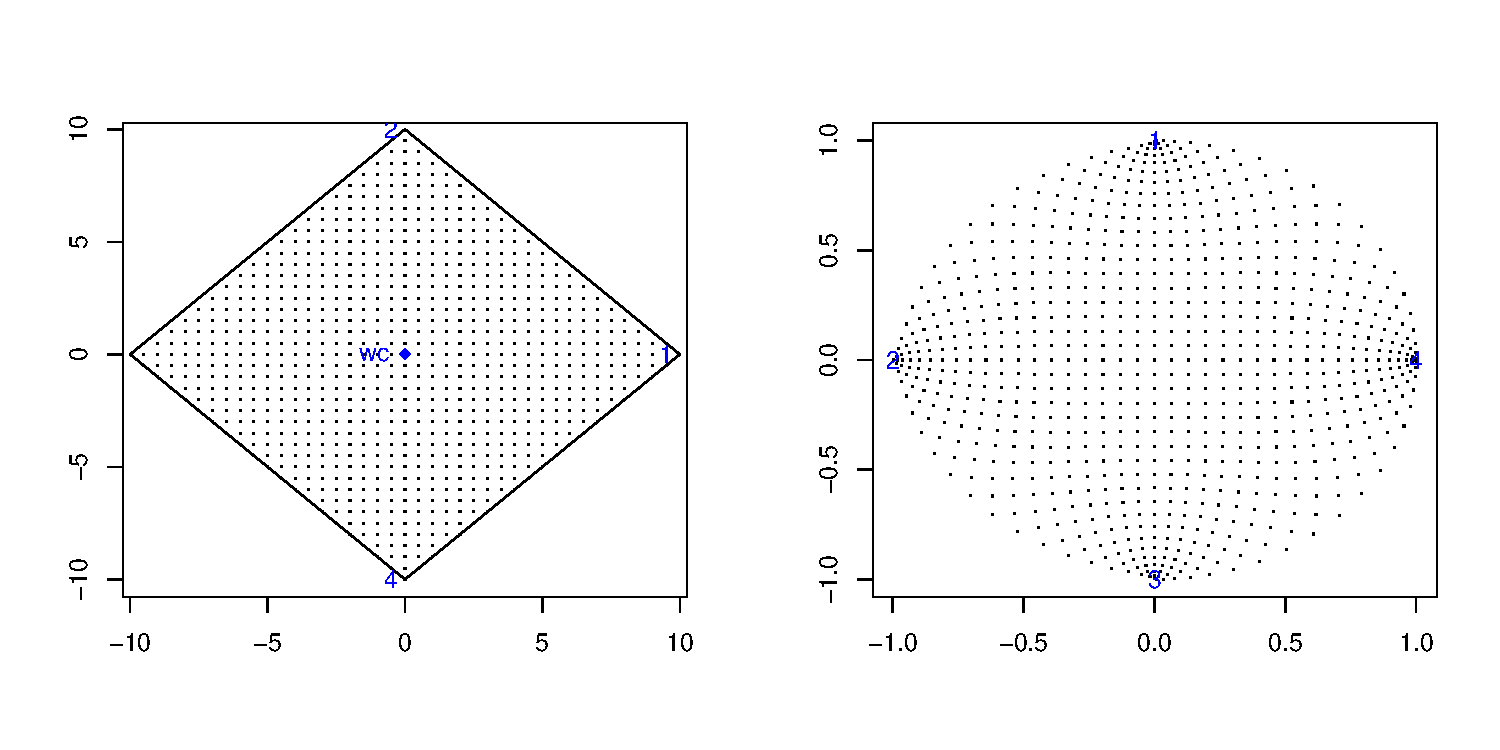
\includegraphics[scale=0.5]{sc/figs/squaredomain.pdf}
\caption{A regular grid of points over the square region (left). The right panel shows the mapping of these points under the \sch\ transformation to the unit disk.}
\label{squaredomain}
\end{figure}

% Irregular mapping diagram
\begin{figure} [tbp]
\centering
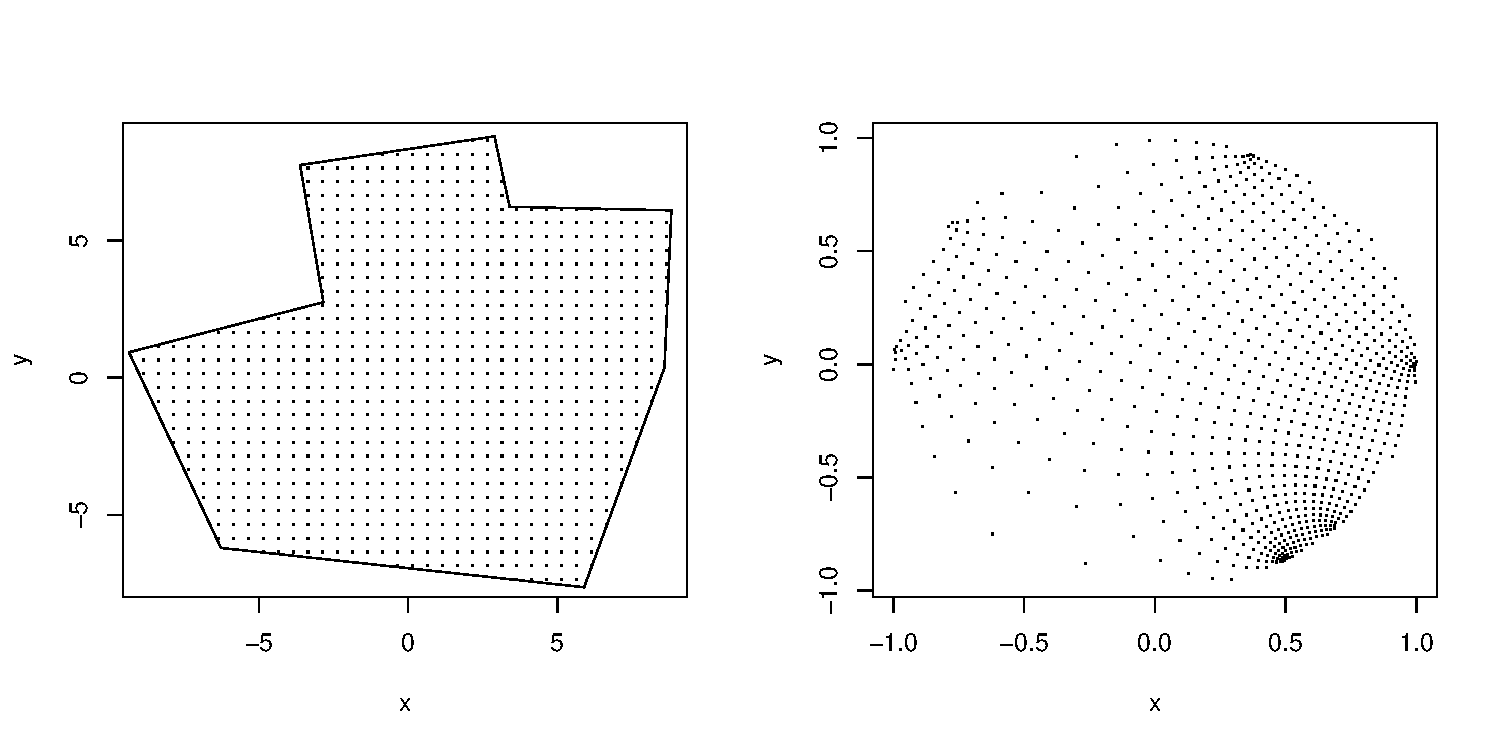
\includegraphics[scale=0.5]{sc/figs/irregulardomain.pdf}
\caption{A regular grid of points over region bound by a irregular nonagon (left). The right panel shows the mapping of these points under the \sch\ tranformation to the unit disk.}
\label{irregdomain}
\end{figure}

\subsection{Crowding}
\label{sch-crowding}

\subsubsection{The crowding problem}
When the polygon is elongated or has many vertices, the mapped vertices may be positioned too closely in the transformed domain. In elongated regions prevertices can be located exponentially close such that they are indistinguishable in finite precision arithmetic (\cite{howell90}). This effect is referred to as \emph{crowding} and can be observed in \fig{crowdeddisk}. 

% Crowded mapping diagram
\begin{figure} [tbp]
\centering
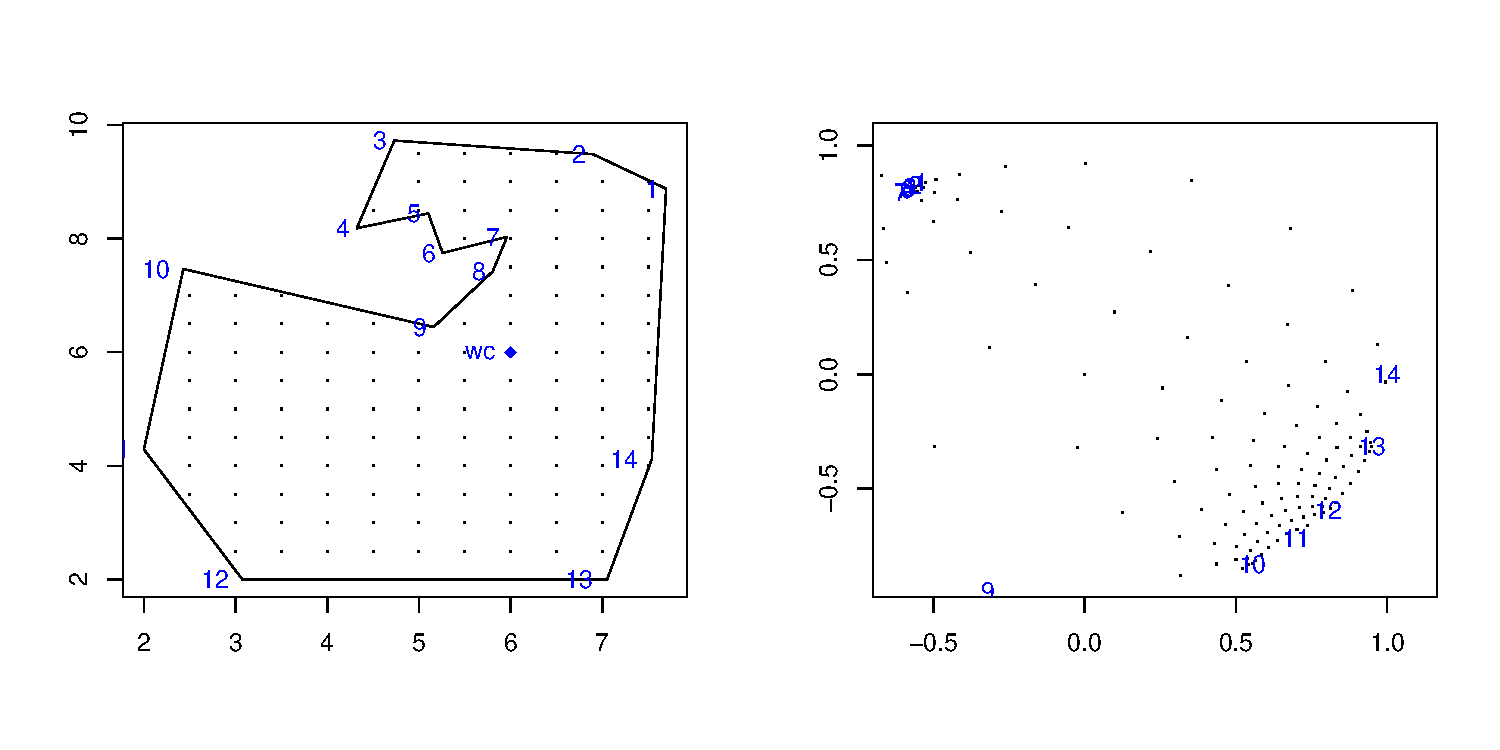
\includegraphics[scale=0.5]{sc/figs/crowdeddisk.pdf}
\caption{An example of crowding. Note that prevertices 1 through 8 are mapped almost to a singularity in the right panel.}
\label{crowdeddisk}
\end{figure}

\subsubsection{Fixing crowding}

If the crowding is caused by $\Gamma$ being elongated then a  primitive fix is to map to an elongated domain such as the rectangle or plane. This approach is suggested in \citeb{howell90}, however, as they point out, this does not eliminate all crowding and problems can still occur when there are acute peninsulae in the polygon. Mapping to an elongated domain also does not fix problems which occur when mapping from T- or H-shaped domains (so-called ``multiply elongated'' domains).

In order to combat this problem more effectively, \citeb{vavasis96} propose the CRDT (cross-ratios of the Delaunay triangulation) algorithm (see below). Each set of prevertices has $K-3$ degrees of freedom, hence there is a three parameter family of possible vertex arrangements that all map to the same polygon. The most stable of these embeddings should be used.

This idea can be extended by noting that the polygon is identical when additional vertices are added between the current ones, provided that the internal angle associated with the new vertex is $\pi$. These extra vertices also do not change the \sch\ formula since in \eqn{unitscmap} $\alpha_k=1$ for an angle of $\pi$. Adding these extra vertices allows us to control the aspect ratio of the mapping.

In the solution to the \sch\ parameter problem given in \secref{sc-parprob}, conditions on the side lengths and orientations of the polygon are enforced. The CRDT algorithm imposes conditions about quadrilateral sections of the polygon and the diagonals of the polygon. First a Delaunay triangulation of the domain is performed and then pairs of triangles are merged into quadrilaterals. A measure is then defined (the \emph{cross-ratio}) which specifies a set of non-linear equations to be solved. These equations enforce the constraint that the cross-ratio in mapped polygon comes out correctly. 

Putting all of these ideas together gives the CRDT algorithm (\cite[pp. 30-39]{driscoll}). First adding edges to the polygon with internal angle $\pi$ to remove elongated parts of the domain and once the domain is triangulated the cross-ratio is found:
\begin{equation}
\rho(a,b,c,d) = \frac{(d-a)(b-c)}{(c-d)(a-b)},
\end{equation}
for each of the $K-3$ quadrilaterals in the polygon (where $a,b,c,d$ are prevertices). Then, analogously to \eqn{optimizeme} a series of equations are set up specifying that the cross-ratios remain the same in the polygon and the transform of the rectangle back to the polygon. Then solving for the values of $\rho$ for the original domain in the same manner as we solved for side lengths in the original problem. 

In \fig{uncrowdeddisk} the CRDT method is used with a rectangular domain, crowding has been alleviated to some degree. The point density, as well as vertex density seems to be more uniform than in \fig{crowdeddisk}.

% Uncrowded mapping diagram
\begin{figure} [tbp]
\centering
\includegraphics[scale=0.5]{sc/figs/irregular-fixed-crdt.pdf}
\caption{The mapping of the irregular domain featured in \fig{crowdeddisk} using the CRDT method mapping to a rectangle. The crowding is now much less severe.}
\label{uncrowdeddisk}
\end{figure}

The downside of using CRDT is that it may add too many vertices to maintain the aspect ratio, so the algorithm takes longer to run than the one specified in \secref{algorithmsketch} since it tends to be cubic in the number of vertices (\cite{driscoll05}). 

\section{Simulation experiments}

In order to test the efficacy of the \sch\ transform for the purposes of smoothing over complex regions, a series of simulation experiments were performed. The \emph{SC Toolbox} for MATLAB was used to perform the transform and the mapping of the points. These were then fed into \textsf{R} and models run using packages \texttt{mgcv} and \texttt{soap}.

\subsection{Ramsay horseshoe}

The most obvious candidate for simulation is the Ramsay horseshoe (see \secref{ramsayfunc}). In order to map as simple a domain as possible, initially a bounding box was used as the $W$ domain remapped via the \texttt{evalinv()} function from the \emph{SC Toolbox}. This is shown in \fig{hswithboundingbox}. The bounding box was then transformed to the rectangle. 

\begin{figure}
\centering
% trim order l b r t
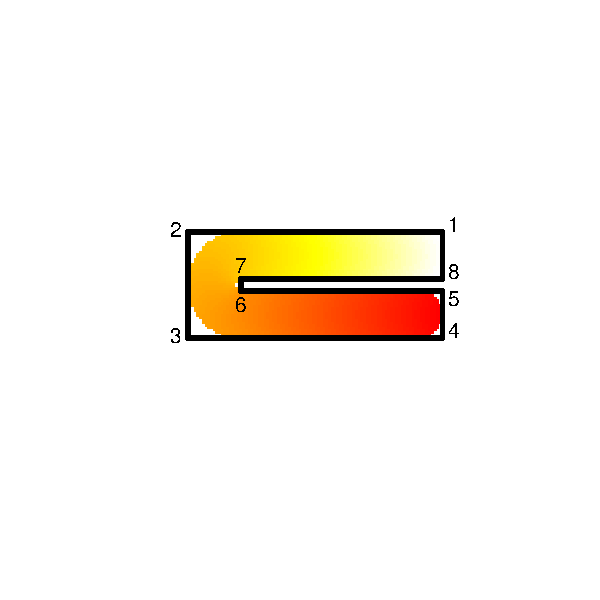
\includegraphics[trim=0.5in 1in 0in 0.5in]{sc/figs/hswithboundingbox.pdf} \\
\caption{The horseshoe with its bounding box. The vertices marked 1, 4, 5 and 8 are mapped to the corners of the rectangle.}
\label{hswithboundingbox}
% generated by /phd-smoothing/sc-writeup/figs/hswithboundingbox.R
\end{figure}

A sample of 1000 points was then taken from the horseshoe and noise added to the data. First the coordinates of the sampled points were expressed as complex numbers of the form (i.e. $w=x_1+ix_2$. The sample was then mapped into $W^*$, creating a new set of coordinates ($w^*=x_1^*+ix_2^*$). Smoothing was then performed over the responses in the $W^*$ domain using the \texttt{gam()} function in \texttt{mgcv}. 

\begin{figure}
\centering
% trim order l b r t
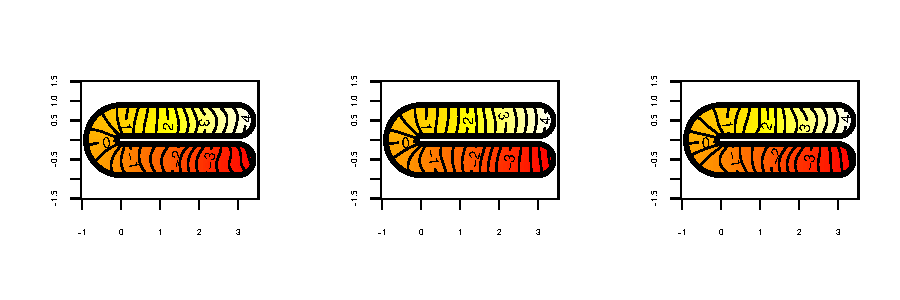
\includegraphics[width=6in]{sc/figs/compsmooth.pdf} \\
\caption{A typical set of predictions using P-splines on the transformed domain (top right), thin plate splines on the transformed domain (bottom left) and soap film smoother (bottom right) for the Ramsay horseshoe (top left). Sample size was 250, the standard deviation of the Gaussian noise added to the samples was set to 1.}
\label{compsmooth}
% generated by figs/pspline.soap.comp.hs.R
\end{figure}

\Fig{compsmooth} shows the true function and typical realisations of: the fit given by a \tprs\ on the transformed domain, a P-spline fit on the transformed domain and the fit given by the soap film smoother. Looking at the heat maps one can see that the general shape of the horseshoe function is clearly being reproduced by all methods (especially in comparison to that in \fig{leakage}). However, on the transformed domains the curvature across the minor axis is not being captured.

\begin{table}[tb]
\centering
\begin{tabular}{c c}\\
Sample size & Noise level \\
\hline
\hline
1000 & 0.3 \\
500 & 0.3 \\
250 & 0.3 \\
100 & 0.3 \\
1000 & 0.5 \\
1000 & 1 \\
1000 & 2 \\
\end{tabular}
\caption{Setup for the simulations using the \sch\ transform for the Ramsay horseshoe. Noise level is the number a random deviate from a standard Normal distribution was multiplied by before being added to the value from true test function.}
\label{scramsimtable}
\end{table}

\Tabref{scramsimtable} shows the settings for noise level and sample size of the simulations. Mean squared error between the true function and the fitted model was used to evaluate the performance of the models. In the following tables we provide the mean squared error over a prediction grid of 1000 points averaged over 1000 generated data sets. The fits on the transformed domain and the soap film have much smaller MSE than the thin plate spline, except in one case, \sch\ with P-splines for sample size 100 and noise level 0.3. Looking closer at the results for this model, there were two results where the MSE was 54.68 and 437.99 which, when removed, put the MSE back to 0.03003, which seems much more reasonable. These results were presumably due to the P-splines' gridded knot setup, giving a poor fit where there was not enough data. This shows one of the many disadvantages of a knot-based approach.

\begin{figure}
\centering
% trim order l b r t
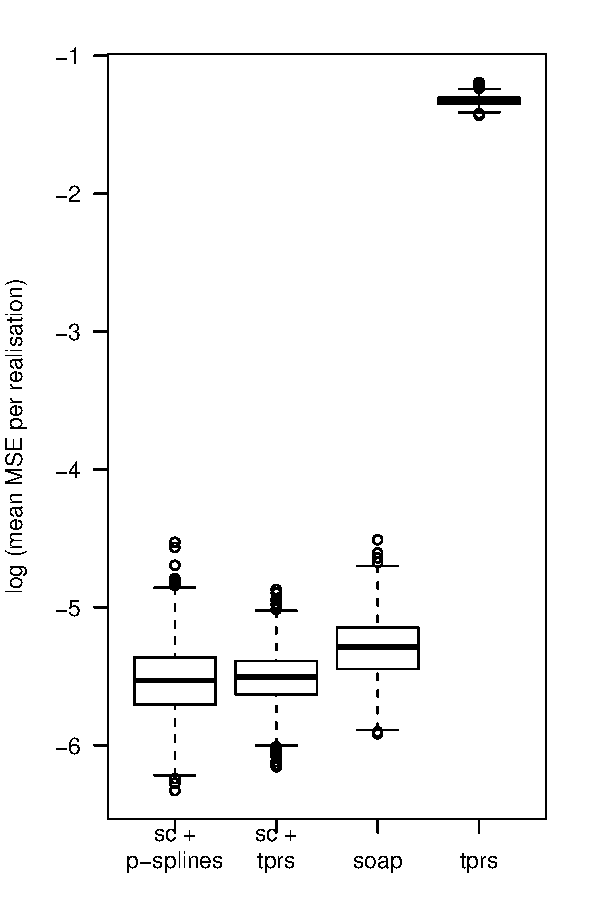
\includegraphics{sc/figs/sc-mses-boxplot.pdf} \\
\caption{Boxplots of the logarithm of mean MSE from 1000 points on a prediction grid from 1000 simulations for the Ramsay horseshoe. Models fitted were \sch\ transform with P-splines and \tprs, the soap film smoother, and \tprs\ (with the untransformed domain). Noise level was set to 0.3.}
\label{scram1000boxplots}
% generated by sc/figs/makeboxplots.R
\end{figure}

\begin{sidewaystable}[hp]
\begin{tabular}{c c c c c c}\\
& & & MSE (se) &\\
Sample size & Noise level & TPRS & SC + P-spline& SC + TPRS & Soap film\\
\hline
\hline
1000 & 0.3 & 0.26611 (0.00029) & 0.00412 (4x10$^{-5}$) & 0.00811 (8x10$^{-5}$) & 0.00517 (4x10$^{-5}$) \\ 
500 & 0.3 & 0.28276 (0.00083) & 0.00505 (6x10$^{-5}$) & 0.00478 (4x10$^{-5}$) & 0.00628 (7x10$^{-5}$) \\ 
250 & 0.3 & 0.32274 (0.00268) & 0.00875 (0.00025) & 0.00684 (0.00012) & 0.01073 (0.00019) \\ 
100 & 0.3 & 0.48371 (0.01765) & 0.52264* (1.39562) & 0.01178 (0.00046) & 0.02194 (0.00117) \\ 
1000 & 0.5 & 0.27336 (0.00032) & 0.01055 (0.00011) & 0.00811 (8x10$^{-5}$) & 0.01268 (0.00011) \\ 
1000 & 1 & 0.30718 (0.00056) & 0.02422 (0.00034) & 0.01607 (0.00022) & 0.02749 (3x10$^{-4}$) \\ 
1000 & 2 & 0.42296 (0.00144) & 0.06596 (0.00152) & 0.03875 (0.00072) & 0.06859 (0.00105) \\ 
\end{tabular}
\label{scramsayres}
\caption{Mean of the mean squared error over 1000 prediction points along with its standard error for the transformed Ramsay horseshoe (for P-spline and thin plate cases) versus those for the soap film smoother. See below for information on the asterisked result.}
% generated by /phd-smoothing/sc-writeup/tablecode/ramsay.sim.results.table.R
\end{sidewaystable}

\Tabref{scramsayres} shows the results from the simulations for the horseshoe. The \sch\ transform yields results which are comparable, it not better, than the soap film. At a sample size of 100 performance degrades for all methods. Although this seems initially encouraging, it is worth bearing in mind at this point that in domains like the horseshoe it is obvious what the transform should be.

Indeed, this can be seen by looking at the predicted values for the model in the $W^*$ domain. \Fig{hsvisgam} shows predictions from the fitted surface alongside the true values when the domain has been put into its ``natural'' coordinate system. The coordinate system for the fitted values is the \sch\ transformed system and for the true values the system is the major and minor axes of the shape (i.e. one axis along the central curve of the shape and the other perpendicular to that). In the plot, the strong linear trend along the major axis of the horseshoe can be seen in both cases, making this a rather trivial smoothing problem. The smooth is being calculated in a close approximation to its natural domain. Such an approximation would not be as easy to find for a less regular, more realistic domain.

\begin{figure}
\centering
% trim order l b r t
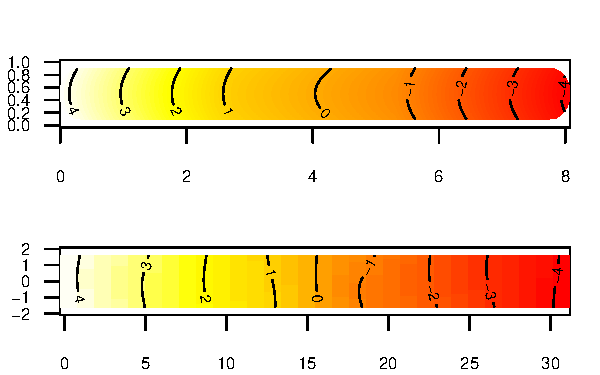
\includegraphics{sc/figs/hsvisgam.pdf} \\
\caption{Heat map of the true values of the modified Ramsay horseshoe projected into its natural domain (left) and the predicted values of the fit given using the \sch\ transform and then smoothed using a \tprs\ (right).}
\label{hsvisgam}
% generated by /phd-smoothing/thesis/sc/figs/hsvisgam.R
\end{figure}

\subsubsection{Alternate Ramsay horseshoe}
\label{sc-alt-horsehoe}
The second domain tested was the alternate version of the Ramsay horseshoe from \citeb{soap}. For this domain there is a ridge running along the major axis of the horseshoe (see \fig{altramsayhorseshoe}). The same simulation setup was used as for the first domain.

\begin{figure}
\centering
% trim order l b r t
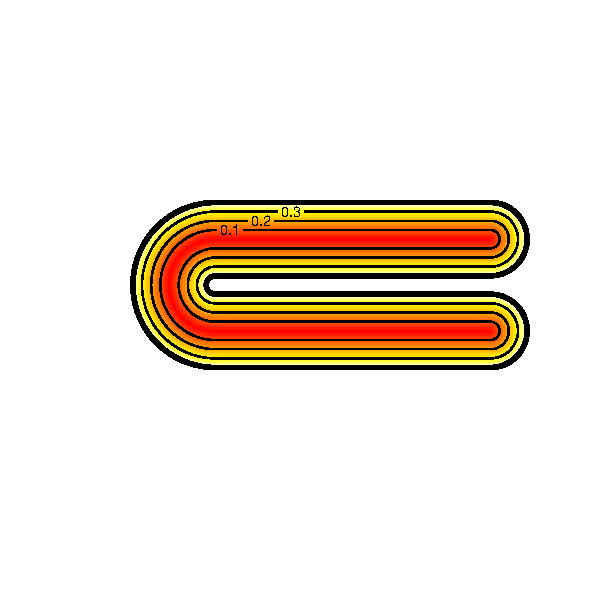
\includegraphics[trim=0.5in 1in 0in 0.5in]{sc/figs/altramsayhorseshoe.pdf} \\
\caption{Heatmap of the alternate version of the Ramsay horseshoe. Unlike the previous horseshoe there is a ridge running along the major axis of the shape.}
\label{altramsayhorseshoe}
\end{figure}

The alternative horseshoe begins to see the soap film creep ahead of the transformation method (see \tabref{scaltramsayresultstable}). Although the MSEs are of approximately the same order (as are the standard errors), the soap film has a lower average MSE for more models now. 

Figure \ref{altramsaycomp} shows that the \sch\ mapping with P-splines captures the overall structure of the shape better than the soap film smoother, which is rather patchy in its reproduction of the alternate horseshoe. Although the P-spline fit ignores the gradient at the ends of the shape. The \sch\ with \tprs\ basis appears worst here, not capturing any of the main features of the domain.

\begin{sidewaystable}[hp]
\begin{tabular}{c c c c c c}\\
& & & MSE (se) &\\
Sample size & Noise level & TPRS & SC + P-spline& SC + TPRS & Soap film\\
\hline
\hline
%1000 & 0.3 & 0.00415 (0.00117) & 0.0158 (0.00247) & 0.00378 (0.00108) \\ 
%500 & 0.3 & 0.00469 (0.00147) & 0.00793 (0.00186) & 0.00458 (0.00145) \\ 
%250 & 0.3 & 0.00716 (0.00431) & 0.0142 (0.00249) & 0.00771 (0.00301) \\ 
%100 & 0.3 & 0.039 (0.22) & 0.0201 (0.00589) & 0.0298 (0.42) \\ 
%1000 & 0.5 & 0.00839 (0.00403) & 0.0158 (0.00247) & 0.00966 (0.00371) \\ 
%1000 & 1 & 0.0194 (0.0122) & 0.0226 (0.0085) & 0.019 (0.00981) \\ 
%1000 & 2 & 0.0605 (0.0468) & 0.0436 (0.0276) & 0.041 (0.0434) \\ 
1000 & 0.3 & 0.0109 (8x10$^{-5}$) & 0.00415 (4x10$^{-5}$) & 0.01579 (8x10$^{-5}$) & 0.00378 (3x10$^{-5}$) \\ 
500 & 0.3 & 0.01395 (1x10$^{-4}$) & 0.00469 (7x10$^{-5}$) & 0.00793 (8x10$^{-5}$) & 0.00458 (6x10$^{-5}$) \\ 
250 & 0.3 & 0.01721 (2x10$^{-4}$) & 0.00716 (0.00027) & 0.01418 (0.00016) & 0.00771 (0.00019) \\ 
100 & 0.3 & 0.0229 (0.00099) & 0.03904 (0.02197) & 0.02011 (0.00059) & 0.02975 (0.04195) \\ 
1000 & 0.5 & 0.01521 (6x10$^{-5}$) & 0.00839 (0.00013) & 0.01579 (8x10$^{-5}$) & 0.00966 (0.00012) \\ 
1000 & 1 & 0.02084 (0.00023) & 0.01943 (0.00038) & 0.02264 (0.00027) & 0.01902 (0.00031) \\ 
1000 & 2 & 0.03843 (0.00072) & 0.06053 (0.00148) & 0.04363 (0.00087) & 0.04096 (0.00137) \\ 
\end{tabular}
\label{scaltramsayresultstable}
\caption{Mean of the mean squared error over 1000 prediction points along with its standard error for the transformed alternate Ramsay horseshoe (for P-spline and thin plate cases) versus those for the soap film smoother. See below for information on the asterisked result.}
% generated by /phd-smoothing/thesis/sc/tablecode/alt.ramsay.sim.results.table.R
\end{sidewaystable}

\begin{figure}
\centering
% trim order l b r t
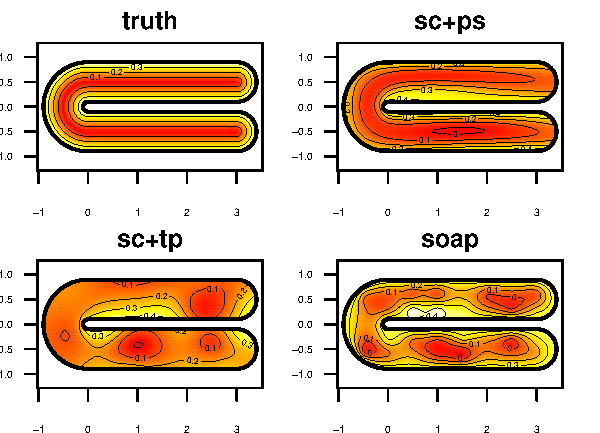
\includegraphics[width=6in]{sc/figs/altramsaycomp.pdf}\\
\caption{Typical realisations of the fit to the alternate Ramsay horseshoe for each method. Clockwise from top left: the original figure, the function estimated by the \sch\ transform with P-splines, function estimated by the \sch\ transform with thin plate splines and finally the soap film estimate. Noise level was 1.}
\label{altramsaycomp}
% generated by /phd-smoothing/sc-writeup/figs/altramsaycompare.R 
\end{figure}


\subsubsection{The effect of the \sch\ transform on the domain}

The \sch\ transform's distortion of the domain causes increase performance of some of the smoothers in some situations but not others. To investigate the effect of the distortion on the domain, the mapping of a straight line in the $W$ domain can be plotted along with its equivalent line in the $W^*$ domain. It is also useful to look at the response along that line in both the transformed and untransformed coordinate systems and see how this compares to looking at the response in the horseshoe's natural coordinate system.

\begin{figure}
\centering
% trim order l b r t
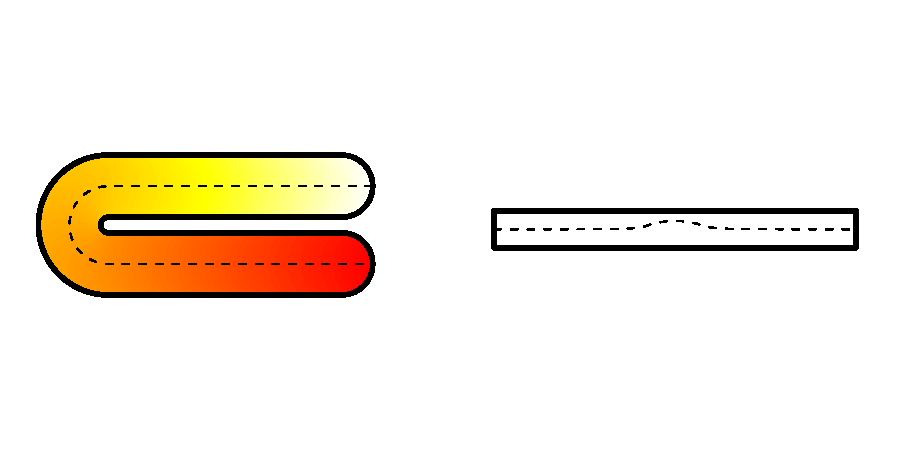
\includegraphics[trim=0.5in 1in 0in 1in]{sc/figs/horseshoecentreline.pdf} \\
\caption{Mapping of a straight line along the major axis of the Ramsay horseshoe to its position in the ``unwrapped'' domain.}
\label{horseshoecentreline}
% generated by /phd-smoothing/thesis/sc/nullspace.test.R 
\end{figure}

\Fig{horseshoecentreline} shows a line along the centre of the horseshoe and its equivalent line in the transformed domain. We can see from this that a line that is straight in the domain (in the sense that it runs parallel to the boundary) has a bump in it in the transform. The curvature does not appear to be particularly extreme in this case, however, one can imagine that this could get significantly worse for regions with more complicated boundaries.

\Fig{centrelinelineplot} shows the evaluations of the horseshoe function along the line plotted against three coordinates. The first plot shows the function evaluations on the $W$ domain as a response to change in $x_2$. The second on the $W^*$ domain, as a response to $x_2^*$, in the transformed coordinate system. The final plot is in the horseshoe's natural domain, i.e. the value the horseshoe takes as a function of distance along the major axis of the shape. From these plots one can see the quality of approximation to the natural domain of the horseshoe the \sch\ transform provides. Only two minor kinks occur in the line. Looking at where the kinks occur, they correspond exactly to those kinks in \fig{horseshoecentreline}. 

\begin{figure}
\centering
% trim order l b r t
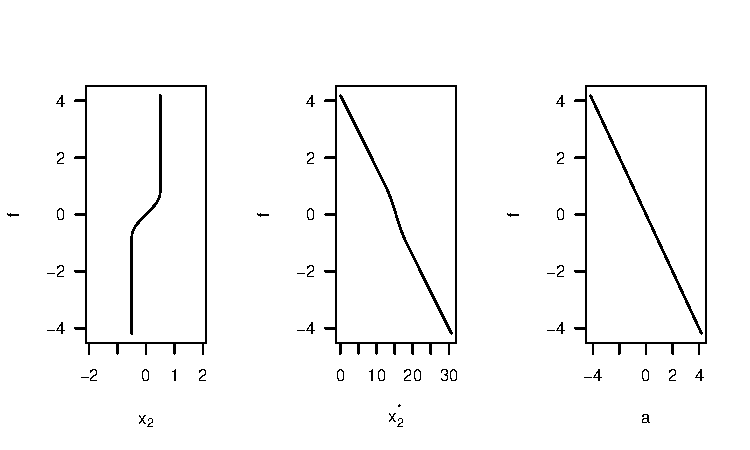
\includegraphics[trim=0in 0in 0in 0in, width=6in]{sc/figs/centrelinelineplots.pdf} \\
\caption{Plots of the horseshoe function against the $y$ axis for (left) the untransformed horseshoe, (middle) the shape under the \sch\ transform and, (right) the function evaluation against the major axis.}
\label{centrelinelineplot}
% generated by /phd-smoothing/ramseysim/nullspace.test.R 
\end{figure}

\Fig{altcentrelinelineplot} shows analogous plots to \fig{centrelinelineplot} for the alternate Ramsay horseshoe and backs up this hypothesis. The second panel shows the mapping of the $x_2$ component of the centreline against the response and the third panel shows the same in the horseshoe's own domain. The two plots appear to be indistinguishable, aside from the change in scale on the horizontal axis.

\begin{figure}
\centering
% trim order l b r t
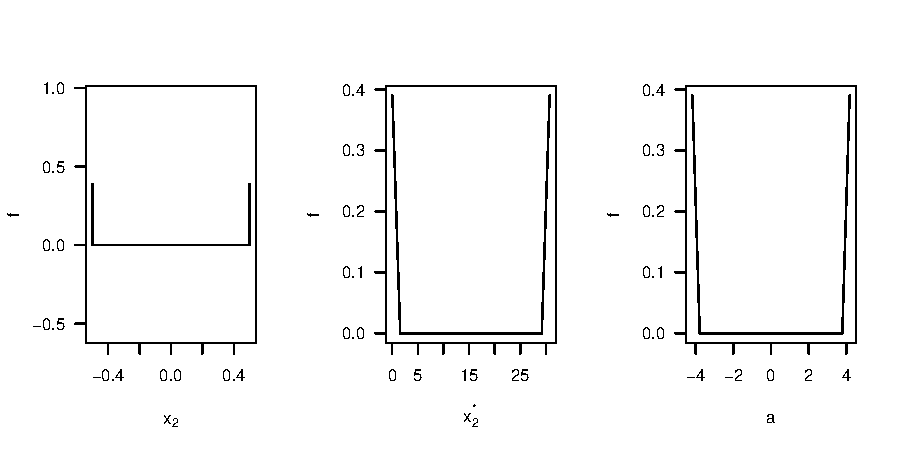
\includegraphics[width=6in]{sc/figs/altcentrelinelineplots.pdf} \\
\caption{Plots of the alternate horseshoe function against the $y$ axis for (left) the untransformed horseshoe, (middle) the shape under the \sch\ transform and, (right) the function evaluation against the major axis.}
\label{altcentrelinelineplot}
% generated by /phd-smoothing/altramsaysim/nullspace.test.R 
\end{figure}

\subsection{Two peninsula domain}

Looking at a more realistic domain highlights potential problems with a \sch\ transform approach. The domain in the top left corner of \fig{sc-wigglytop2-real} shows a domain which is supposed to replicate some of the features of such a domain.

% realization
\begin{figure}
\centering
% trim order l b r t
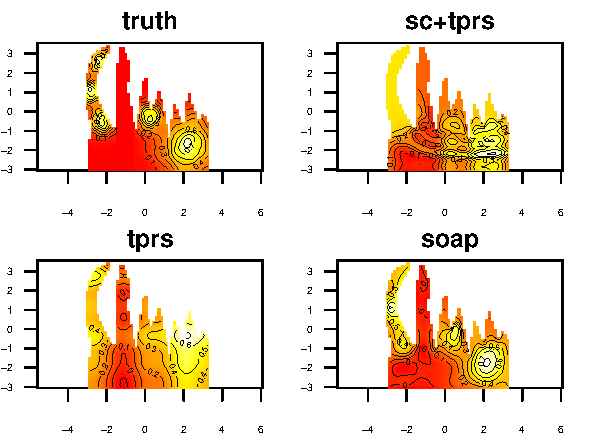
\includegraphics[width=6in]{sc/figs/wigglytop2-real.pdf} \\
\caption{The peninsulae domain. From top left, clockwise: truth, fit from \sch\ transform with \tprs, soap film smoother fit, and \tprs\ fit for typical realisations. Sample size was 500 and the noise level was 0.02. For the \sch\ transformed domains, the rectangular mapping was used.}
\label{sc-wigglytop2-real}
% generated by wigglytop2 fit.irregular.R
\end{figure}

The CRDT algorithm was used for the \sch\ mapping, extra vertices introduced into the polygon with angle $\pi$, are shown, along with the mapping in \fig{wigglytop2-numbered}. From this figure one can see that although there is no crowding in the numerical sense of \citeb{driscoll}, there is significant ``bunching-up'' of the vertices. This would indicate that odd artefacts might be introduced into the smooth.

Several combinations of vertex mappings and knots were tried. The result of this was that the vertices chosen to map to the corners of the rectangle were those shown in pink in \fig{wigglytop2-numbered}. For the soap film smoother a 15 by 15 grid of internal knots was used, of which 109 were inside the region. The cyclic spline around the boundary used 49 knots. Clearly this is the kind of domain in which the soap film smoother performs well (when the chance of leakage is high).

% wt2 vertex mapping
\begin{figure}
\centering
% trim order l b r t
\includegraphics{sc/figs/wigglytop2-numbered.png} \\
\caption{Mapping of the polygon to rectangle for the double peninsula domain example. Note the extra vertices added by the CRDT algorithm.}
\label{wigglytop2-numbered}
% generated by Matlab
\end{figure}

% wt2 point mapping
\begin{figure}
\centering
% trim order l b r t
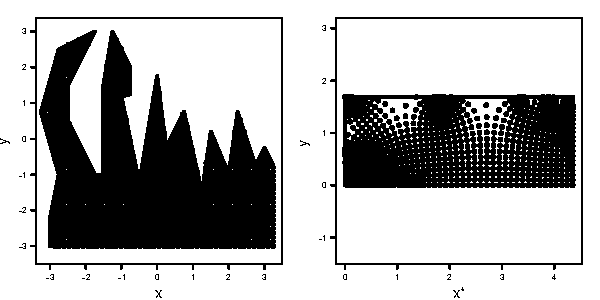
\includegraphics[width=6in]{sc/figs/wt2-points.pdf} \\
\caption{Change in the density of points between the mapped and unmapped spaces for the double peninsula domain. Areas with particularly high density in the right panel correspond to vertices in the left.}
\label{wt2-points}
% generated by thesis/sc/figs/wt2-pointmap.R
\end{figure}

Looking at the realisations in \fig{sc-wigglytop2-real}, one can see that the \sch\ transform causes a huge distortion in the surface. The contour lines in the upper right pane of the figure show how the distortions have pushed the data points around, causing a very bad fit. It also looks as though there is a ridge across the smooth over the domain, which is clearly unwanted. The \tprs\ and the transform method both smooth over the details in the first peninsula. The soap film smoother is vastly superior to either method in this situation as can be seen in the boxplots in \fig{wigglytop2-boxplots}.

% boxplot
\begin{figure}[p]
\centering
% trim order l b r t
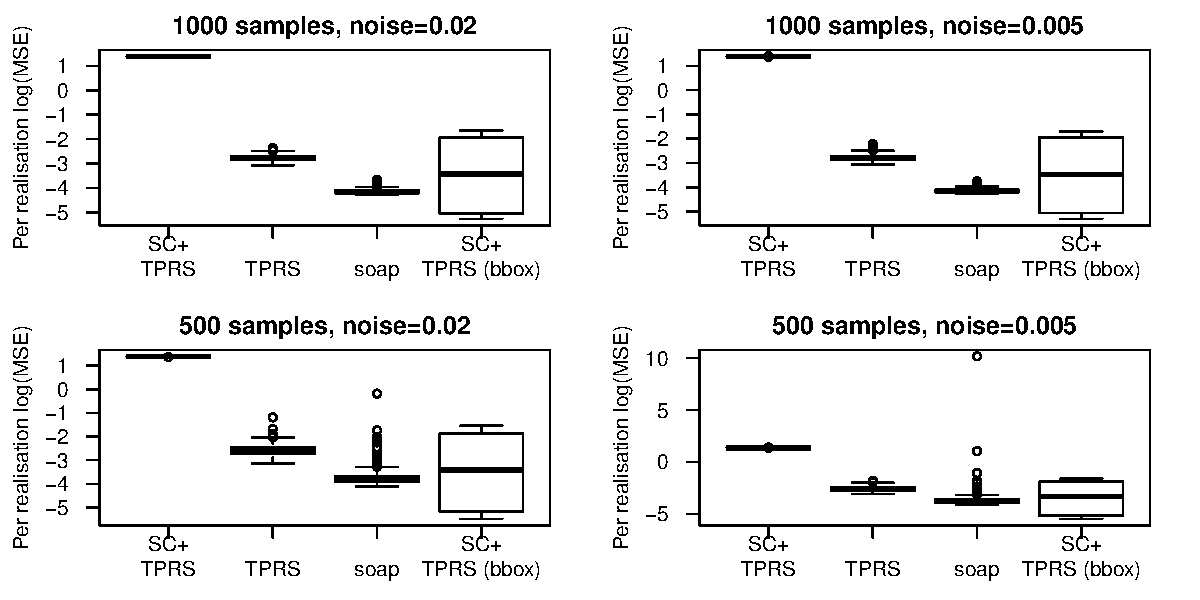
\includegraphics[width=6in]{sc/figs/wigglytop2-boxplot.pdf} \\
\caption{Boxplots of the logarithm of the MSE averaged over 1253 prediction points for 500 replicates for the rectangle mapping and the bounding box mapped to the rectangle, alongside the soap film smoother and \tprs.}
\label{wigglytop2-boxplots}
% generated by makeboxplots.R
\end{figure}

\Fig{wigglytop2-boxplots} also shows the results of using the simpler bounding polygon shown in \fig{wigglytop2-bbox-numbered} with the \sch\ mapping (again mapping to the rectangle) as  an attempt to reduce the distortions seen in \fig{sc-wigglytop2-real}. Although the median $\log(\text{MSE})$ was reduced, there was a massive increase in variability; there is no significant increase in performance by attempting to use the bounding polygon. Although this ironed out some of the artifacts in the smooth, \fig{wigglytop2-bbox-real} shows that new features appear. It appears that the \sch\ transform does not perform well in such a situation.

\begin{figure}[t]
\centering
% trim order l b r t
\includegraphics[width=3in]{sc/figs/wigglytop2-bbox-numbered.png} \\
\caption{The CRDT mapping of the bounding box to the rectangle for the peninsula domain. Pink vertices correspond to those mapped to the corners of the rectangle.}
\label{wigglytop2-bbox-numbered}
% generated by Matlab
\end{figure}


% realisation
\begin{figure}
\centering
% trim order l b r t
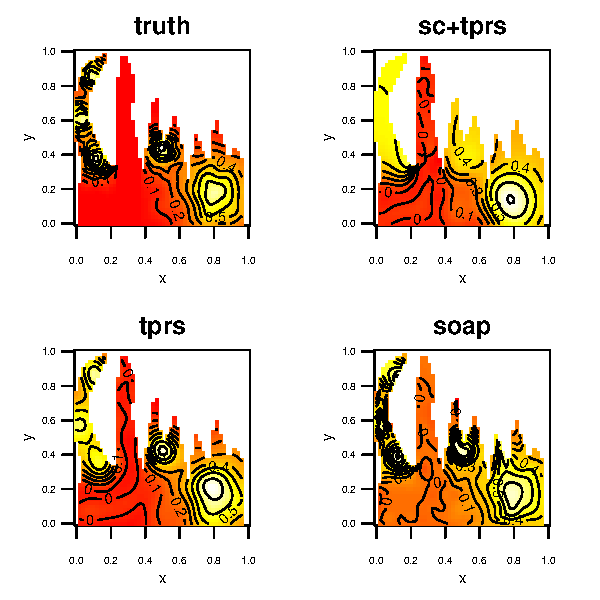
\includegraphics[width=6in]{sc/figs/wigglytop2-bbox-real.pdf} \\
\caption{The domain with two peninsulae. Truth and typical realisations for (clockwise from top right) a \tprs\ fit to the \sch\ transformed domain using the bounding box, the soap film smoother, and a \tprs\ on the untransformed domain. Sample size was 500 and the noise level was 0.02.}
\label{wigglytop2-bbox-real}
% generated by wigglytop2-bbox fit.irregular.R
\end{figure}


\section{Conclusions}
\label{sc-conclusions}

Domain morphing-type techniques undeniably show some promise when it comes to the problem of smoothing over complex regions. Yet the \sch\ mapping is not the correct transformation to use for  all domains. What has been seen here is that the mapping is too prescriptive in its morphing of the domain. There is nothing special about the shape that the polygon is morphed to, it is just a convenient shape to smooth over. The restriction to only use the unit disk, rectangle, etc. constrains the technique, causing phenomena which are as bad (if not worse) than the leakage we initially wanted to avoid.

Crowding (in a technical sense) can be avoided by using the CRDT algorithm, but the spatial inhomogeneity caused by using the \sch\ transform is still a stumbling block for smoothing. This, fundamental problem of mapping between domains is exacerbated by using a restricted set of shapes to map into. It would be preferable to minimise the distortion to the distribution of points in space and using a less regular domain for $W^*$, rather than having a pre-specified domain, which causes the spatial inhomogeneity.

The point map in figure \ref{wt2-points} shows that the \sch\ transform can clearly split the domain, drawing apart those areas of the domain which were causing the leakage previously. In the case of the Ramsay horseshoe, the transformation that is needed is obvious. Problems occur when the transformation is not obvious. With the peninsula domain, it is not clear what an appropriate domain to map into would look like even if the \sch\ transform could map to an arbitrary shape. Certainly, the rectangle or unit disk are not the shapes which immediately come to mind.

Fortunately, all is not lost. This brief foray into conformal mapping has provided plenty of insights into how smoothers will act under mapping schemes. It has also given an appreciation of the criteria which dictate the utility of a transformation-based method, especially with regard to how smoothing behaves when space is distorted.

With these points in mind, the next step is to find a general mapping scheme for domains with complicated boundaries which is not too prescriptive, causes minimum distortions to the distribution of space but minimises the effects of leakage.



